\section{Graph Networks}

\subsection{Message Passing Neural Networks}

Gilmer et al. describes Message Passing Neural Networks (MPNN) as a framework that generalizes at least eight models found in the literature ~\cite{Gilmer_2017}. The MPNN method describes a messaging and a readout phase on forward propagation.
	
The hidden nodes, $h_v^t$, are updated based on messages $m_v^{t+1}$, for a number of timesteps.

\begin{equation}
    \label{eqn:message}
    m^{t+1} = \sum_{w \in N(v)} M ^ {T} (h^t_v, h^t_w, e_{vw})
\end{equation}

\begin{equation}
    h^{t+1} = U_t(h^t_v, m^t_v)
\end{equation}

\begin{equation}
    \hat{y} = R (\{h^t_v | v \in G\})
\end{equation}

\begin{itemize}

    \item The message function, $M^{t}$, plays the role of the GN’s $\phi ^ e$, but does not take $u$ as input,
    
    \item Element wise summation is used for the GN’s $\rho ^ {e \rightarrow v}$,
    
    \item The update function, $U_t$, plays the role of the GN’s $\phi ^ v$
    
    \item The readout function, $R$, plays the role of the GN’s $\phi ^ u$, but does not take $u$ or $E'$ as input, and thus an analog to the GN’s $\rho ^ {e \rightarrow u}$ is not required;
    
    \item $d_{\text{master}}$ serves a roughly similar purpose to the GN’s $u$, but is defined as an extra node connected to all others, and thus does not influence the edge and global updates directly. It can then be represented in the GN’s $V$.

\end{itemize}

\begin{figure}[!htb]
    \centering
    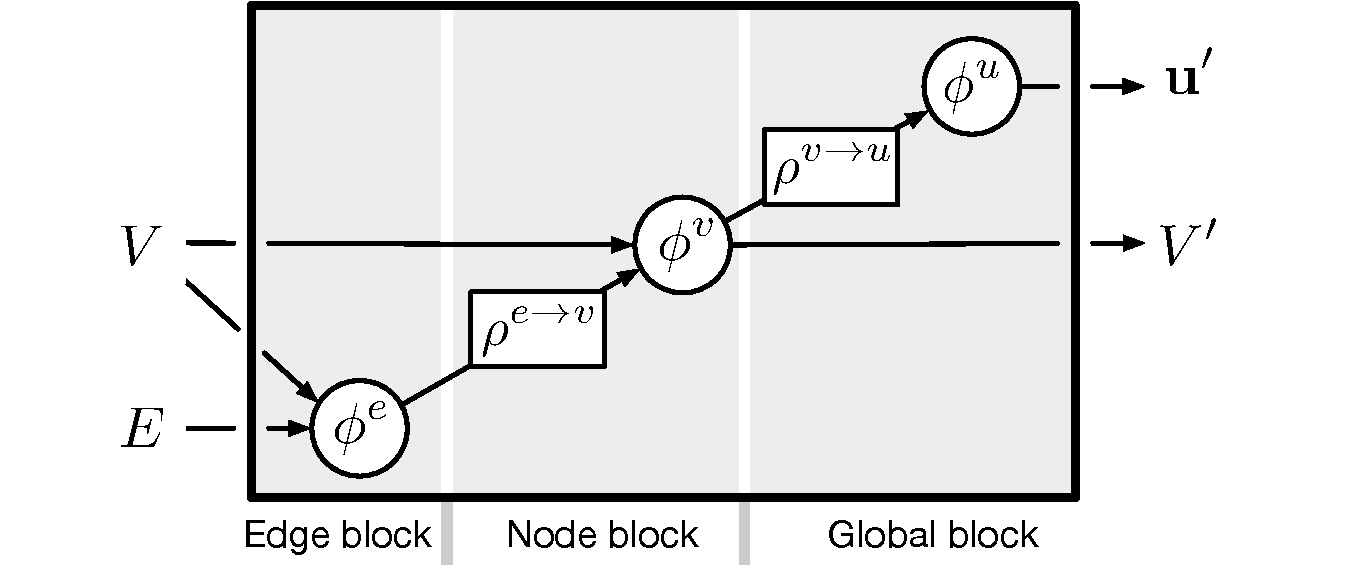
\includegraphics[height=3.0cm]{fig/content/graph_nets/blocks/mpnn.pdf}
    \caption{The forward pass phases of the Message Passing block elicited above ~\cite{Battaglia_2018}.}
\end{figure}



\subsection{Non Local Neural Networks}

Both recurrent and convolutional operations are building blocks that process one local neighborhood at a time. On the other extreme, fully connected layers have those relations encoded in the learned weights, therefore the relationship between the points is not a direct function of the input layer. 

Non Local Neural Networks (NLNN), ~\cite{Wang_2018} presents a mid-term building blocks for capturing long-range dependencies.

In it, the forward pass is computed by repeatedly applying a weighted sum of a function of the previous step, but in this case part of the weight is a similarity measure between the node being calculated and the node being summed over.

\begin{equation}
    h^{t+1}_v = 
    \cfrac{1}{C(h^t)} 
    \cdot \sum_{\forall u \in V} {
        f(h^t_v,h^t_u) \cdot g(h^t_u)
    }
\end{equation}

\begin{figure}[!htb]
    \centering
    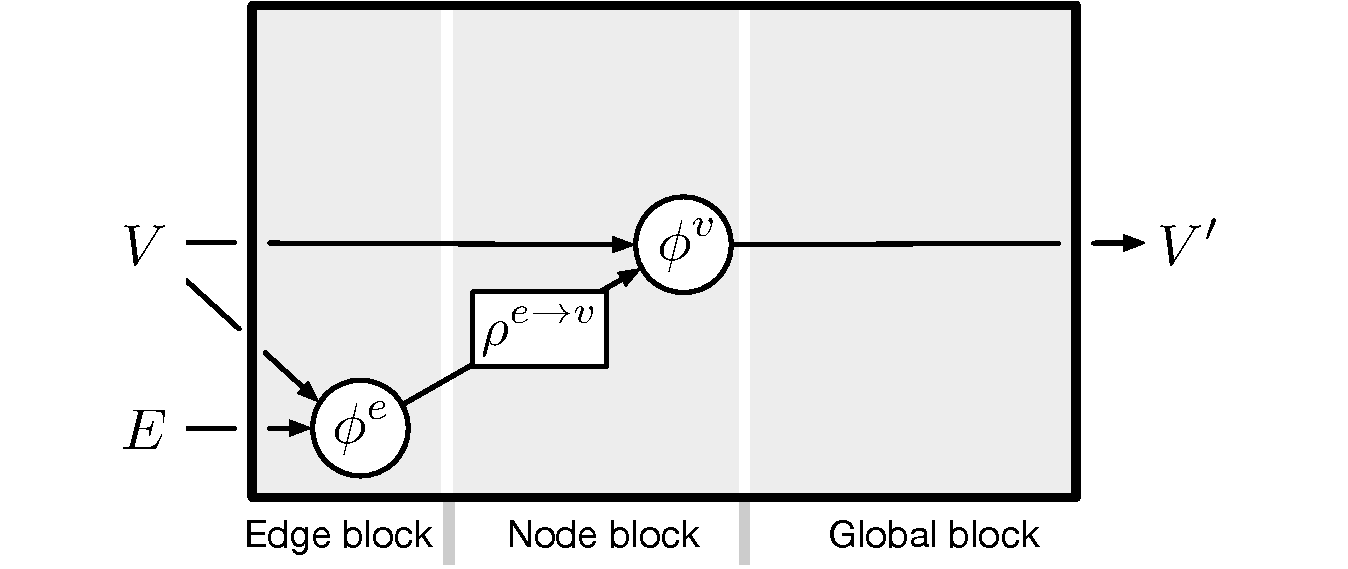
\includegraphics[height=3.0cm]{fig/content/graph_nets/blocks/nlnn.pdf}
    \caption{The forward pass phases of the Non Local Neural Network block ~\cite{Battaglia_2018}.}
\end{figure}

\subsection{Graph Independent}

The Graph Independent module applies models to the graph elements independently, i.e., the models are applied to each element of the graph (nodes, edges and globals) in parallel regardless of other elements.

\begin{figure}[!htb]
    \centering
    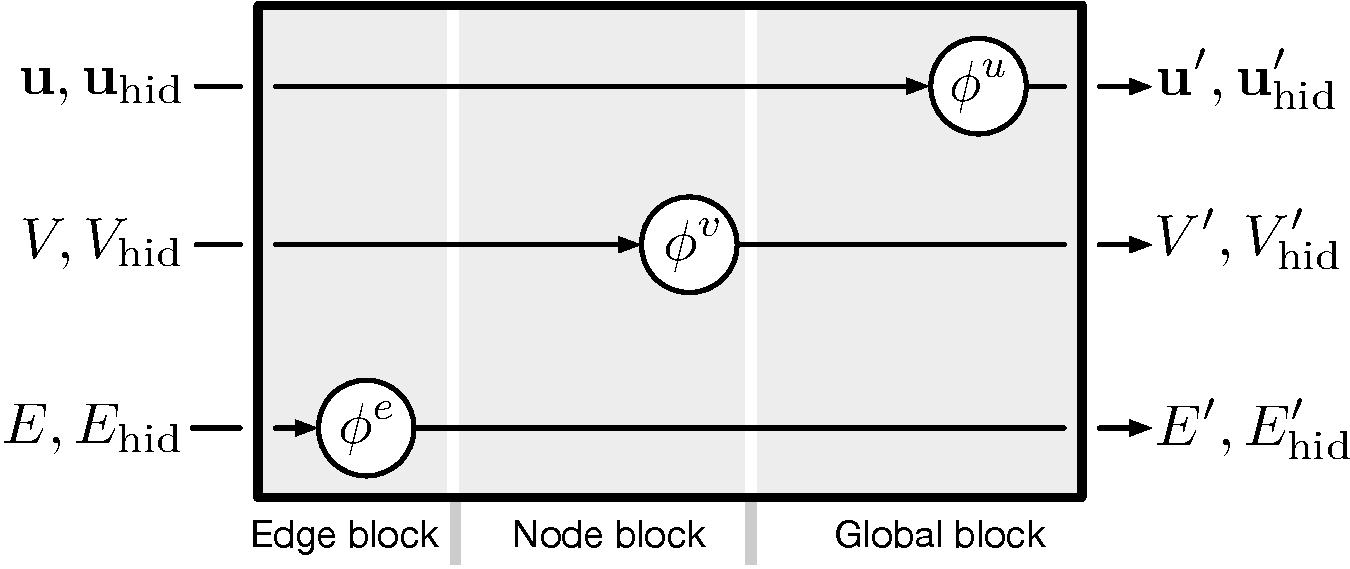
\includegraphics[height=3.0cm]{fig/content/graph_nets/blocks/independent.pdf}
    \caption{The forward pass phases of the Graph Independent block ~\cite{Battaglia_2018}.}
\end{figure}

\subsection{Graph Nets}

The Graph Networks (GN) framework generalizes and extends various graph neural network approaches, such as MPNN and NLNN (Non Local Neural Networks) ~\cite{Battaglia_2018}. A Graph Net is composed of blocks which operate a sequence of steps according to its configuration. One possible configuration, a full GN block (a), predicts node, edge, and global features based on its incoming nodes, edges, and global features.

Graph Nets framework encompasses flexible representations, configurable in-block structure and composable multi-block architectures ~\cite{Battaglia_2018}. This is shown in the example block arrangements in (Fig. \ref{fig:graph_nets_flexibility}) In each block, $\phi$ (phi) functions may be applied to incoming attributes and $\rho$ functions to aggregate them, generating new, updated output values (shown as either $u'$, $V'$ or $E'$).

\begin{figure}[!htb]
    \centering
    \subfigure[Full block]{
        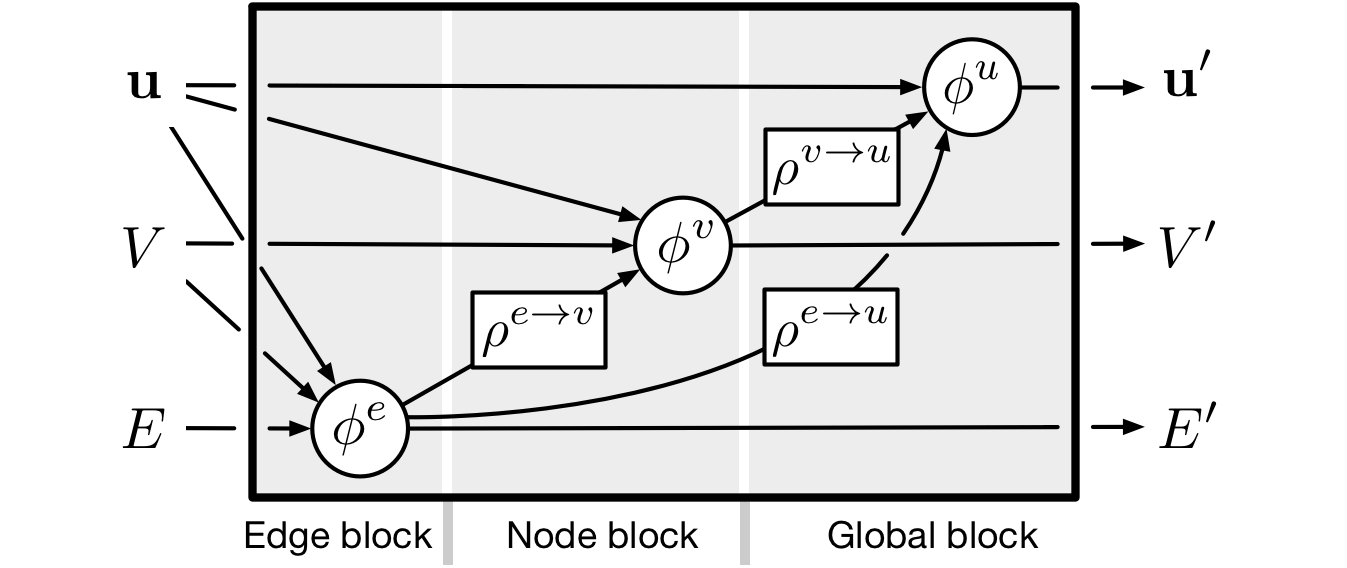
\includegraphics[width=.45\linewidth]{fig/content/graph_nets/blocks/full.png}
    }
    \subfigure[Independent block]{
        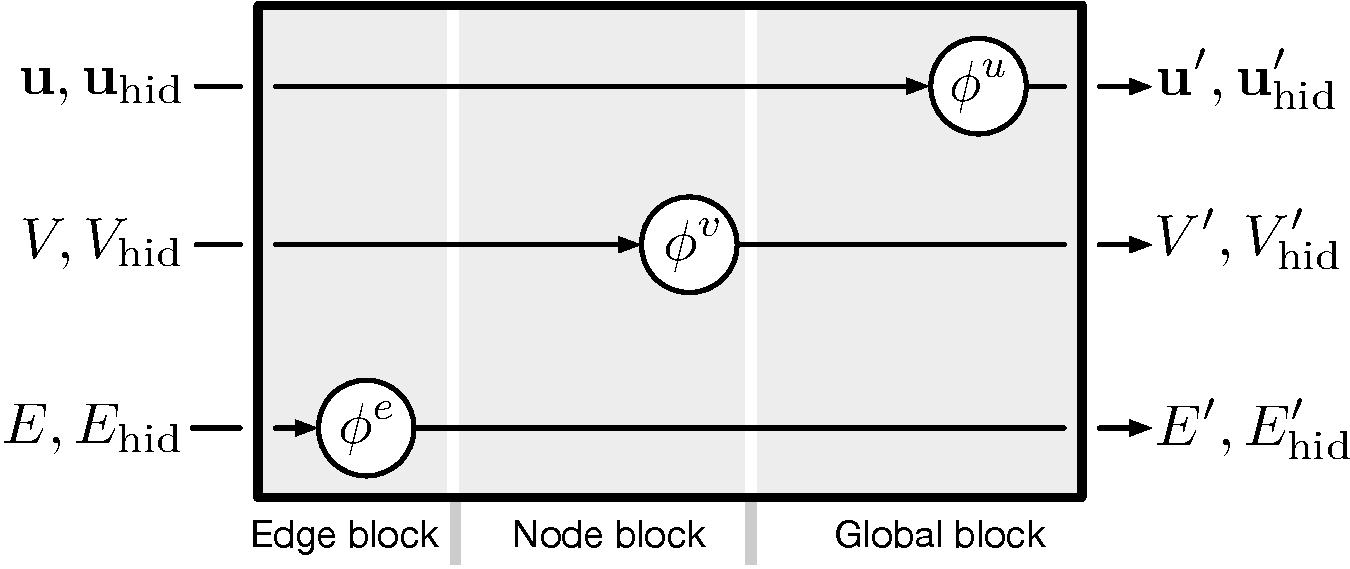
\includegraphics[width=.45\linewidth]{fig/content/graph_nets/blocks/independent.pdf}
    }
    \subfigure[Message-passing block]{
        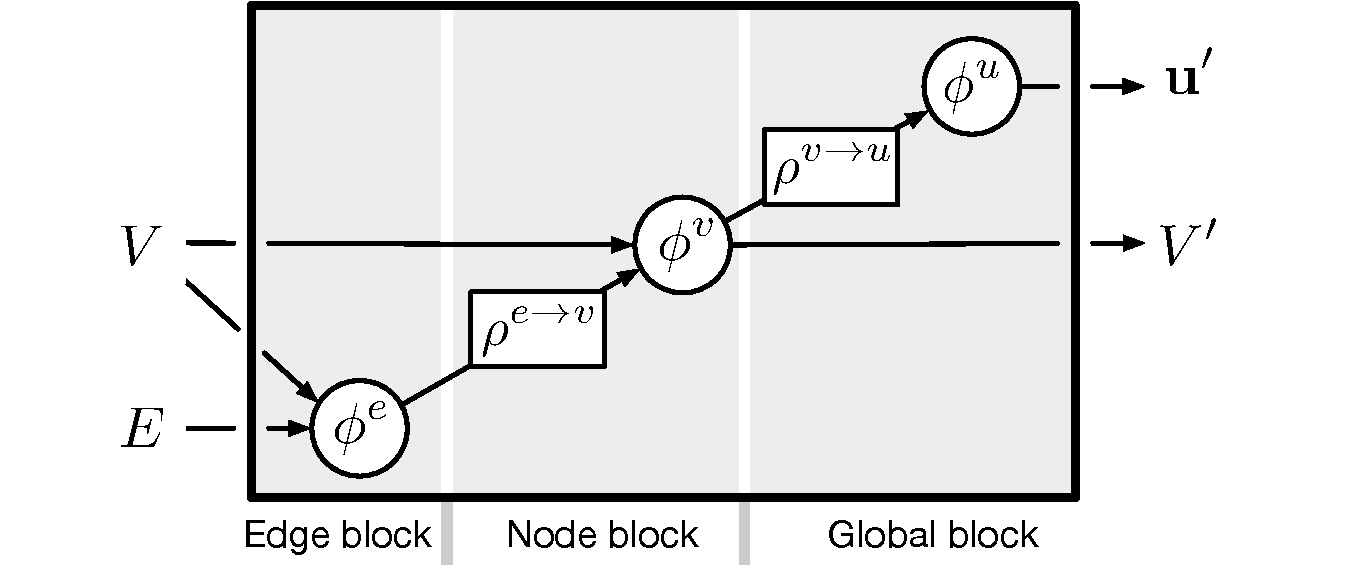
\includegraphics[width=.45\linewidth]{fig/content/graph_nets/blocks/mpnn.pdf}
    }
    \subfigure[Non Local block]{
        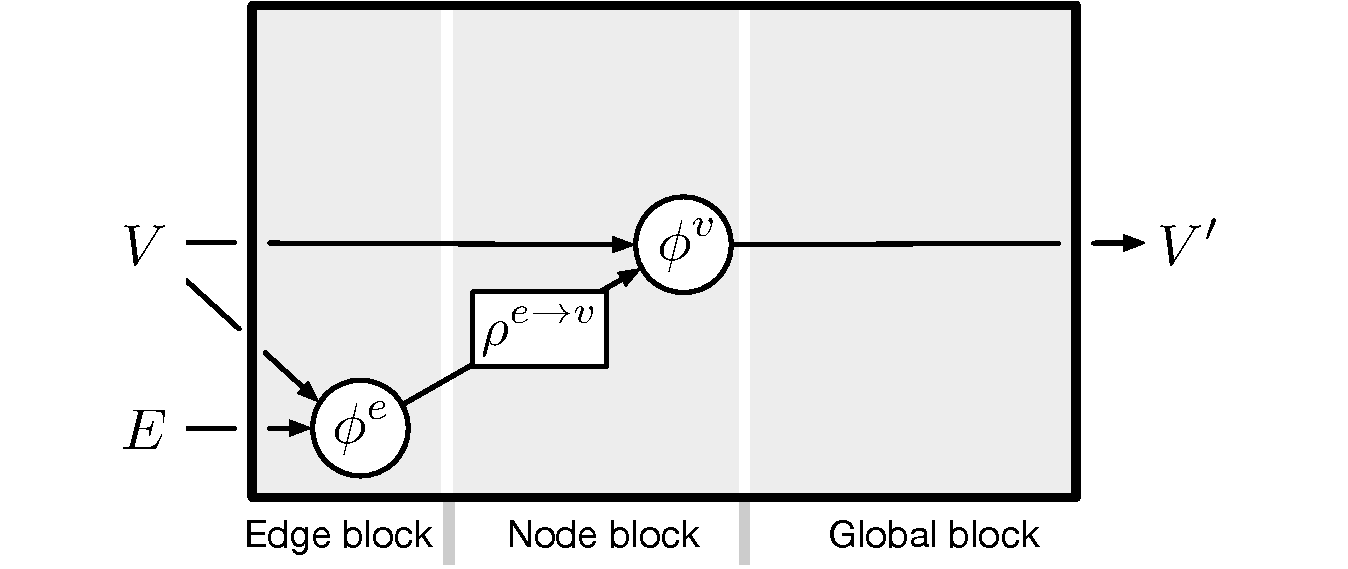
\includegraphics[width=.45\linewidth]{fig/content/graph_nets/blocks/nlnn.pdf}
    }
    
    \caption{Graph Nets internal block configurations ~\cite{Battaglia_2018}}
    
    \label{fig:graph_nets_flexibility}
\end{figure}




\section{Analyzed Problems}


\subsection{State Prediction of a Spring-mass System}

This problem explores a computational simulation derived from an actual physics experiment. Given a set of masses connected one another by springs, with two of them fixed, e.g. pinned to a wall, the problem is to predict the next state of the masses after  some noise was applied.

The state of the masses is defined as a 2-D position and velocity. The system always starts from rest position, with all masses in the same vertical position and zero velocity in the two dimensions. They also start with the same distance apart from one another.

A computational simulation of this system was carried out by Battaglia et al. (2016)'s "interaction networks" ~\cite{Bataglia_2016} using deep learning and more recently in ~\cite{Battaglia_2018}. In the simulation, a random dataset is generated by initializing nodes with fixed spacing among them, and then applying noise on every timestep.

In the system, masses are translated into nodes and springs into edges. This produces a graph where each non-fixed node has two adjacent neighbors. The vertex feature vector is composed by the tuple $(x, y, v_x, v_y, \text{fixed})$, where $x$, $y$ denote position, $v_x$, $v_y$ denote velocity and fixed denotes whether a mass is fixed.

The edges’ feature vector is composed by the springs’ rest distance and their constants. The global feature vector is composed solely by the gravitational acceleration, which is -10m/s².

The model generates a trajectory by applying noise at each iteration of the simulation. By the end, a graphs dataset is ready to be input into the neural network. Training data examples have 5 to 8 masses, while test data have 4 to 9 masses.

\begin{figure}[!htb]
    \centering
    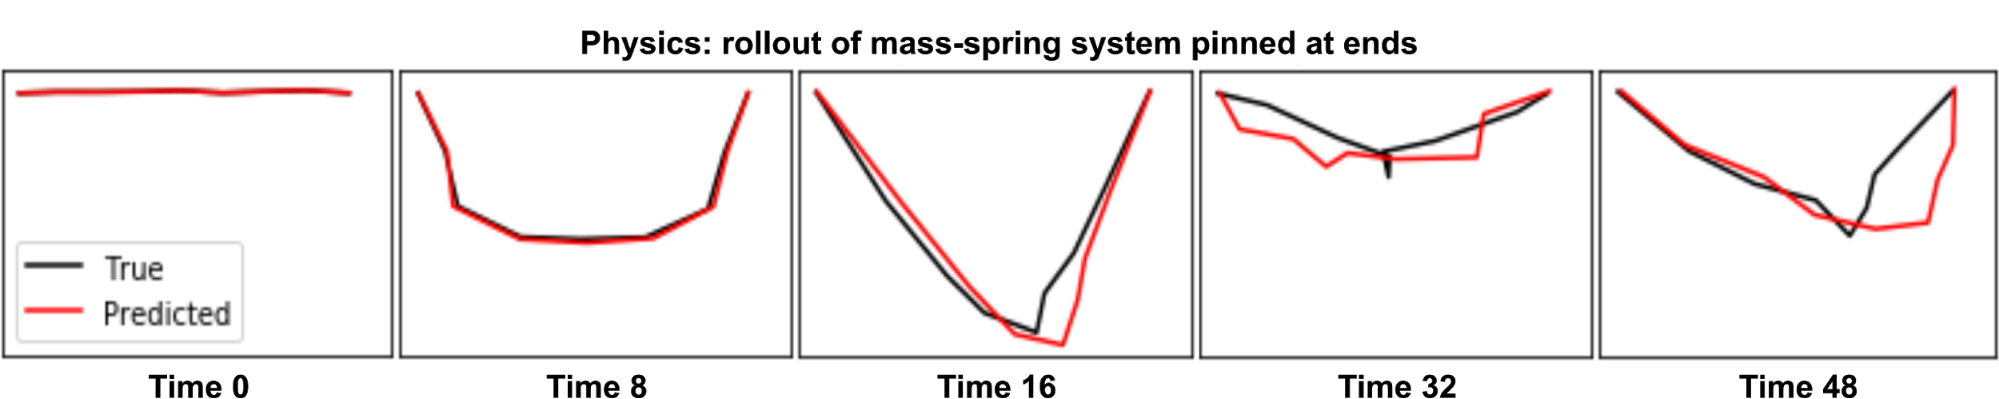
\includegraphics[height=3.0cm]{fig/content/analysed_problems/physics/tragectory.png}
    \caption{Predicted and true values from states along a spring-mass trajectory ~\cite{Battaglia_2018}.}
\end{figure}


\subsection{Shortest Paths}

The experiment creates random graphs, and trains a graph network to label the nodes and edges on the shortest path between any two nodes. Over a sequence of message-passing steps, the model refines its prediction of the shortest path.

\begin{figure}[!htb]
    \centering
    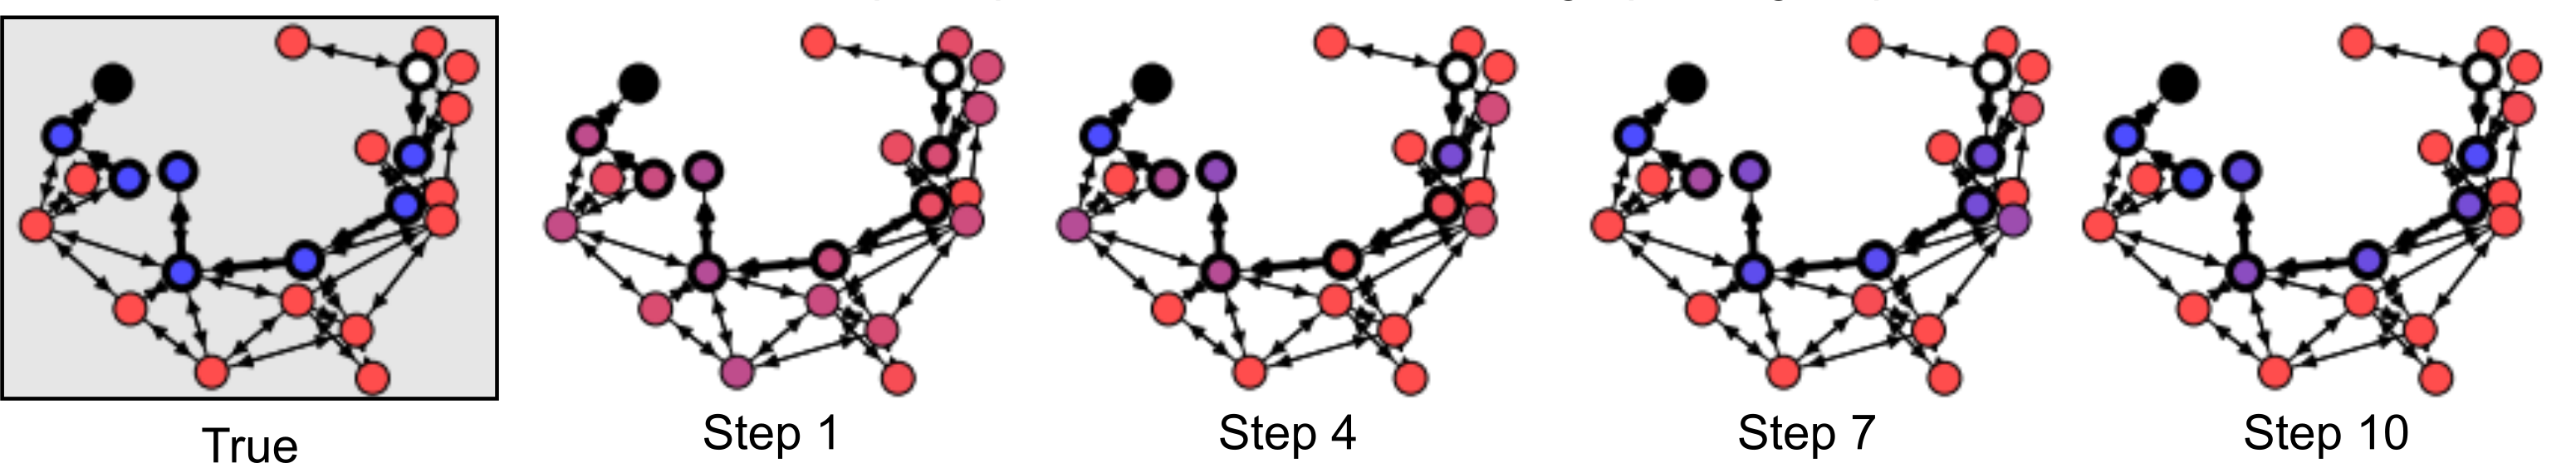
\includegraphics[height=3.0cm]{fig/content/analysed_problems/shortest_paths/steps.png}
    \caption{Prediction at each message-passing step for shortest path problem ~\cite{Battaglia_2018}.}
\end{figure}


\subsection{Regions Separation}

The problem here is the classification of pixels of an input image, given its similarities with its neighbors. 

At first glance, this problem might not seen related with a graph to graph problem, but we can make a reduction of this problem to one of finding a set of independent connected components that represent each of the different classes of pixels. 

So the input is transformed into a graph network with one vertex for each pixel and a link of two vertices if the corresponding pixels are neighbors.

The output can be transformed simply by partitioning the graph with a Depth First Search (DFS) or using the vertex class feature that the reduced problem must also provide.

The problem that we explored is the reduced one: Given the graph network described and exemplified below, with features indicating color and position in each vertex, produce the graph with vertices of different regions in different connected components and with features indicating in what region the vertex is. Since the set of edges in the solution is always a subset of the edges in the input, we used an edge feature to indicate if the corresponding edge is part of the solution.

\begin{figure}[H]
    \centering
    
    \subfigure[Input image and associated graph]{
        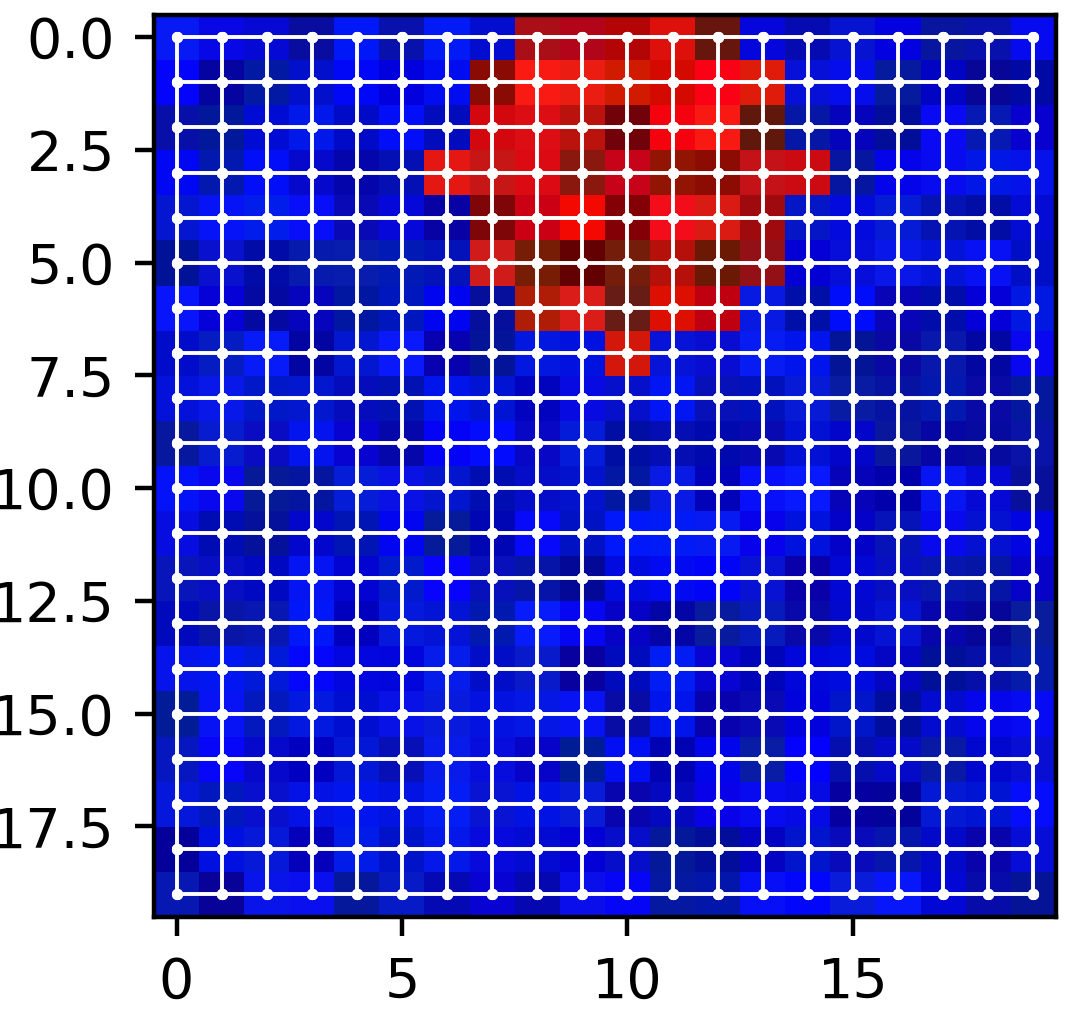
\includegraphics[width=.45\linewidth]{fig/content/analysed_problems/shapes/input.png}
    }
    \subfigure[Expected image and associated graph]{
        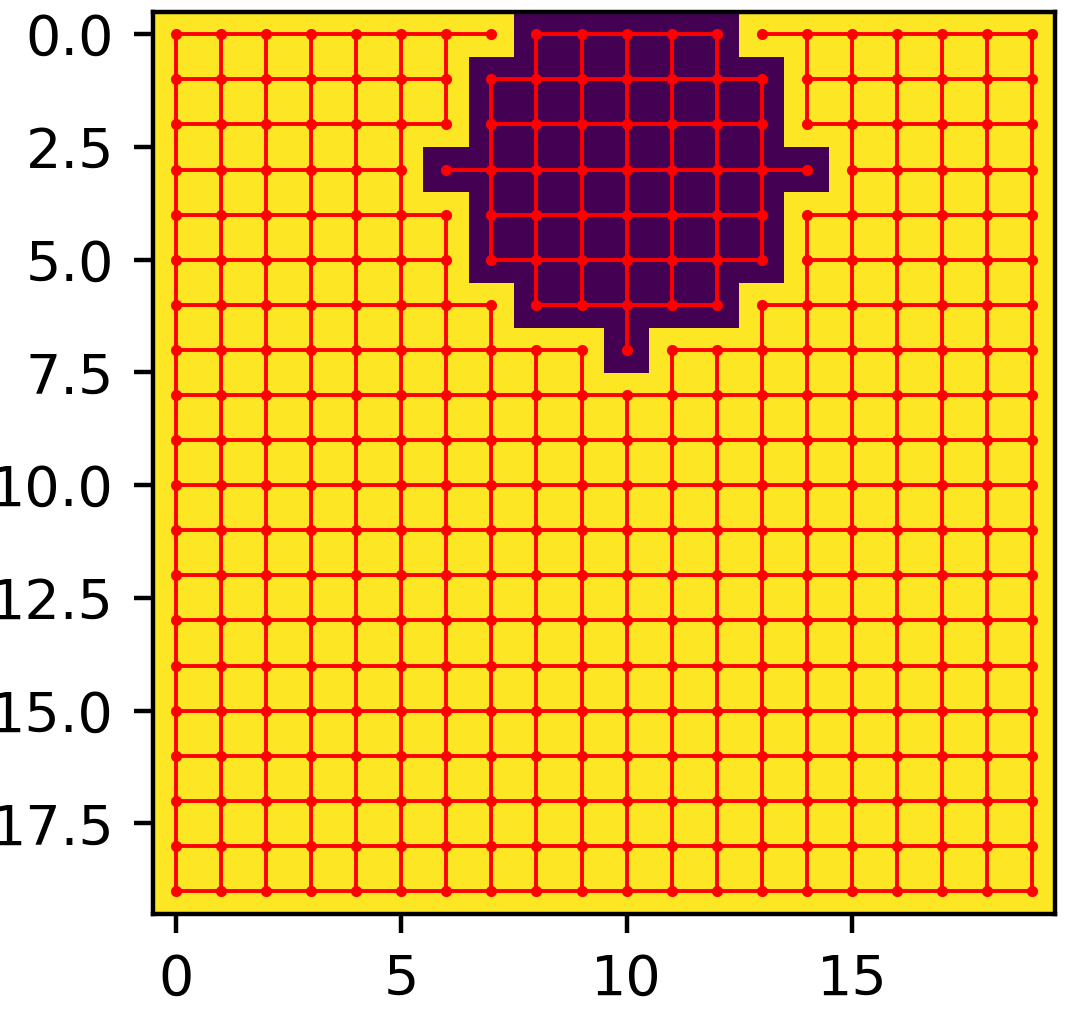
\includegraphics[width=.45\linewidth]{fig/content/analysed_problems/shapes/expected.png}
    }
    
    \caption{Visualization of an entry of the dataset used for the Region Separation problem}
    
    \label{fig:regions_separation_dataset_visualization}
\end{figure}


\section{Methodology}

\subsection{The Model}

The experiments used a full encode-process-decode model. That is, the model included three components:

\begin{itemize}

    \item Encoder: the Graph Independent module, which independently encodes the nodes, edges and global attributes
    
    \item Core: the Graph Network (GN) module, which performs N rounds of message-passing processing steps. The input is the concatenation of the Encoder’s output and the Core’s previous output.
    
    \item Decoder: the Graph Independent module, which independently decodes nodes, edges and global attributes on each message-passing step.

\end{itemize}

The model looks like this:

\begin{figure}[!htb]
    \centering
    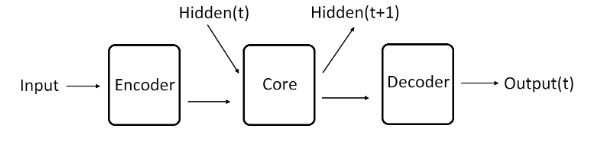
\includegraphics[height=3.0cm]{fig/content/model/model.jpg}
    \caption{The model}
\end{figure}

We used supervised learning to train the model. 

The training loss is computed on the output of each processing step. This encourages the model to try to solve the problem in as few steps as possible, and helps the output of intermediate steps to be more interpretable.

The testing loss is computed only on the final processing step and evaluates how well the model generalizes to graphs that are larger than those it was trained.

The experiments consisted of:

\begin{enumerate}[label=(\Alph*)]

    \item Training on non-permuted data and testing on both non-permuted  and permuted data.
    
    \item Training on permuted data and testing on both non-permuted and permuted data.

\end{enumerate}

\subsection{Physics Experiments}

The experiments followed the baseline model described by (A) and (B).

The default parameters were used, i.e. learning rate $10^{-3}$, a $10^5$ training iterations, with test being applied every 20 seconds, training batch size 256 and test batch size 100.

In (A) the permutation was applied as a branch from the original test dataset, but with permuted node feature vector and senders/receivers.

In (B) the permutation was applied during training graphs’ generation.

Sum of squared error was applied to determine loss at each evaluation. Accuracy was not calculated.

\subsection{Shortest Paths Experiments}

The graphs are geographic threshold graphs with add edges (using a minimum spanning tree algorithm) to guarantee that all nodes are connected. Then, attributes that indicates the shortest path from A to B are added to the graph. From this graph, called raw graph, we get the source and target graphs which are fed to the model described above.

The training graphs have a range of number of nodes from 8 to 17, and for the testing graphs we have a range of 16 to 33. The batch sizes are 5, for training, and 100, for testing.

The loss were computed using Softmax Cross Entropy from TensorFlow. The optimizer we used were the Adam Optimizer, also from TensorFlow. And for the learning rate we used $10^{-3}$. These were the default parameters used by the model from Graph Nets.

\subsection{Regions Separation Experiments}

To produce the input graph, we first generate an image consisting of two shapes in different colors with a random noise applied to the whole image.

The input graph nodes are created for each pixel of the image and from each pixel is extracted horizontal and vertical position along with red, green and blue channels as node features.

The input graph edges are created by connecting vertices with adjacent pixels (vertically and horizontally, not diagonally).
The target graph is a similar network, but with edge features indicating if the respective edge is part of the solution.

An edge is considered to be part of the solution if the two corresponding pixels are from the same region of the image, if they have the same color before the applied noise or, in other words, if it is not in the separation of the two shapes.

The training graphs have the number of nodes taken from a uniform distribution in the range from 8 to 17, and for the testing graphs we have a range of 16 to 33. The batch sizes are 5, for training, and 100, for testing. We used an epoch with 25 iterations, testing every 3 iterations in a simple and a permuted graph. In total the algorithm ran through 125 iterations, so 5 epochs. This is all repeated with 5 different seeds.

The loss were computed using Softmax Cross Entropy from TensorFlow. The optimizer we used were the Adam Optimizer, also from TensorFlow. And for the learning rate we used $10^{-3}$.

\section{Results and Discussion}

For the Loss graphics, we used:

    \begin{itemize}
        \item Ltr: training loss
        \item Lge: testing/generalization loss
        \item Lpe: permuted testing/generalization loss
        \item Lge4: testing/generalization loss with 4 masses
        \item Lpe4: permuted testing/generalization loss with 4 masses
        \item Lge9: testing/generalization loss with 9 masses
        \item Lpe9: permuted testing/generalization loss with 9 masses
    \end{itemize}
    
And for the Accuracy graphics, we used:

    \begin{itemize}
        \item Str: training graphs solved correctly
        \item Sge: testing/generalization graphs solved correctly
        \item Spe: permuted testing/generalization graphs solved correctly
        \item Ctr: training graph elements correctly labeled
        \item Cge: testing/generalization graph elements correctly labeled
        \item Cpe: permuted testing/generalization graph elements correctly labeled
    \end{itemize}

\subsection{Experiments A - Physics}

\subsubsection {Permutation of the testing set}

This experiment was carried out to compare the network’s performance between testing against a dataset and its permuted version. The results of this setup are shown in Fig.\ref{fig:physics_base_results} with a logarithmic scale indicating the training and test losses (both baseline and permuted).

The Loss graphic (Fig.\ref{fig:physics_base_results}) exhibits higher loss for Lpe4 and Lpe9 curves (permutation test). The permutation loss curves kept above the 100 mark during all the training, while the baseline loss curves kept as high as 10 or less on average. This indicates an increase in difficulty to detect next states when the network had to deal with permuted data.

An explanation for this is that the network may have learned well to identify some key features. For example, it may have learned the fixation of the first and last masses, as of the order of input of nodes, and derived the spring-mass pattern for trajectory projection for intermediate nodes.

\begin{figure}[H]
    \centering
    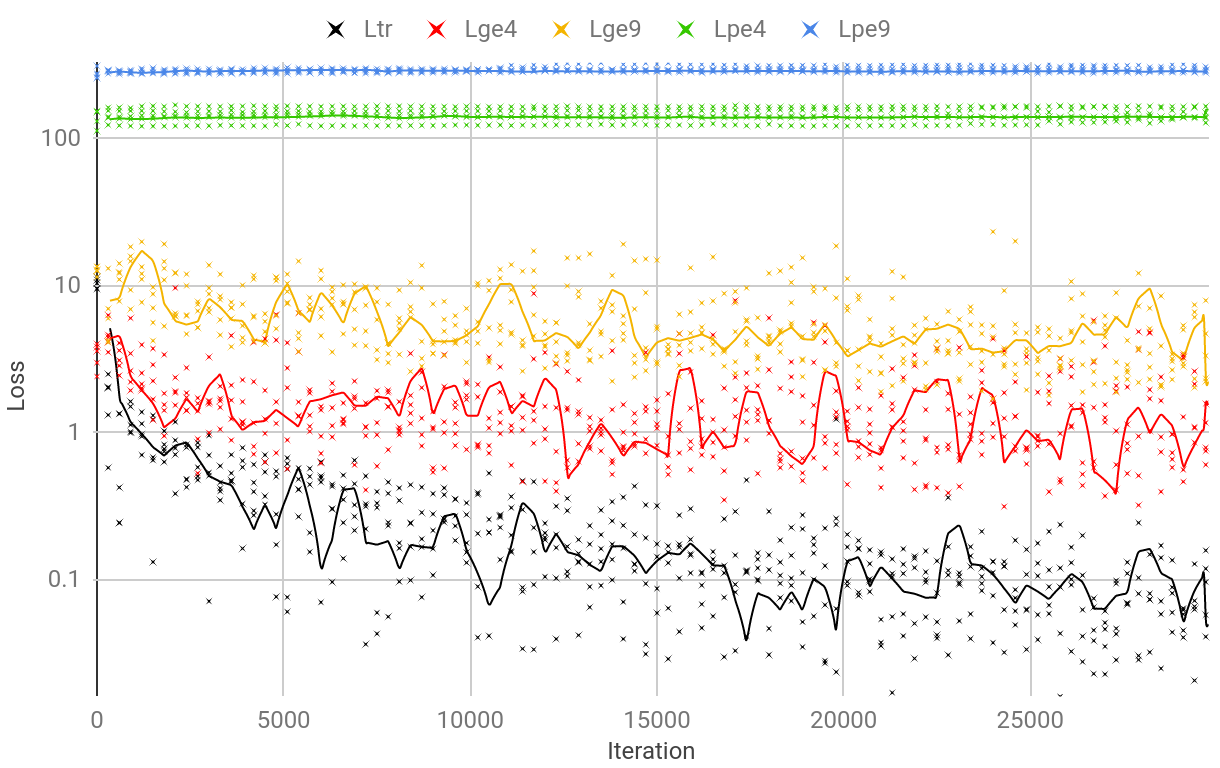
\includegraphics[width=.9\linewidth]{fig/content/results/physics/physics_base.png}
    \caption{Loss graphic of the physics experiment with permutations only of the testing set}
    \label{fig:physics_base_results}
\end{figure}

\subsubsection {Permutation of the training and testing sets}

This experiment evaluated the algorithm’s performance on raw test data and permuted test data after training with permutations.

The results displayed in the Loss graphic (Fig.\ref{fig:physics_perm_results}) show smaller differences between raw test data and permuted test data. These results indicate the algorithm is actually learning and optimizing for permuted test data as well.

An explanation for this phenomenon is that the use of randomness for determining the position of masses in the system input (implemented as nodes) increases the generalization capability of the network.

\begin{figure}[H]
    \centering
    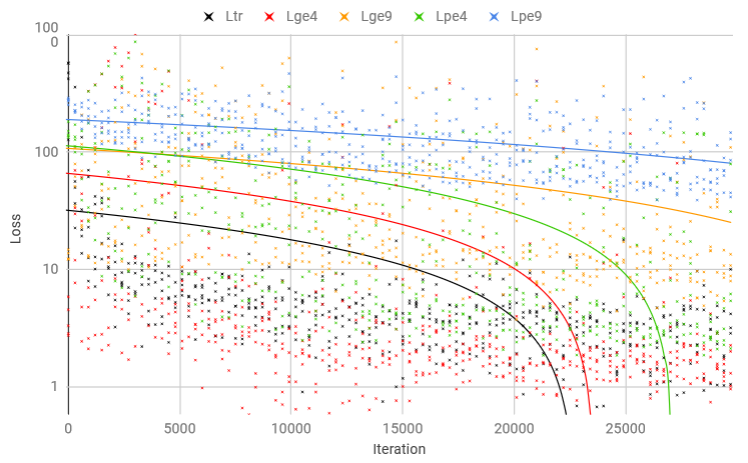
\includegraphics[width=.9\linewidth]{fig/content/results/physics/physics_perm_minium_squares.png}
    \caption{Loss graphic of the physics experiment with permuted training and testing sets}
    \label{fig:physics_perm_results}
\end{figure}

\subsection{Experiments B - Shortest Paths}

The experiments were done with different SEEDs (the graphs were randomly generated with the SEEDs), and with different configurations:

\subsubsection {Permutation of the testing set}
    \begin{enumerate}[label=(\Alph*)]

        \item Infinite dataset
        \label{sec:infinite_test_only}
        
        An infinite dataset were used for the training and testing sets, at each iteration new graphs were randomly generated to train and test the network. The testing set were evaluated with and without permutations.
        
        The Loss graphic (Fig.\ref{fig:shotest_paths_base_results}) shows that the loss of the permuted testing set is the highest and, different from the loss of the non-permuted testing set, is not decreasing after iteration 75.
        
        And in the Accuracy graphic (Fig.\ref{fig:shotest_paths_base_ACC_results}) we can see that the network does not learn to identify the shortest path on the permuted testing set (the trend of the permuted testing set's accuracy is far from 1).
        
        \begin{figure}[H]
            \centering
            \includegraphics[width=.9\linewidth]{fig/content/results/shortest_path/base.png}
            \caption{Loss graphic with infinite training set with permutations only of the testing set}
            \label{fig:shotest_paths_base_results}
        \end{figure}
        
        \begin{figure}[H]
            \centering
            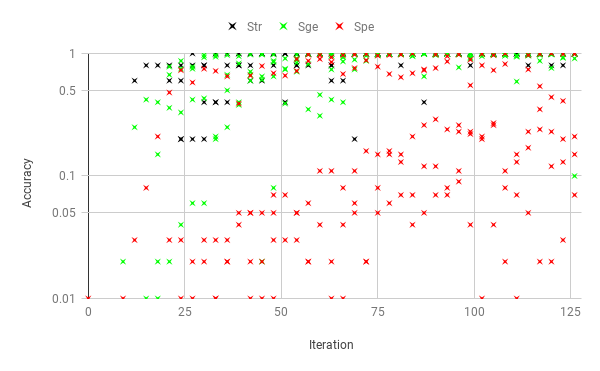
\includegraphics[width=.9\linewidth]{fig/content/results/shortest_path/base_ACC.png}
            \caption{Accuracy graphic with infinite training set with permutations only of the testing set}
            \label{fig:shotest_paths_base_ACC_results}
        \end{figure}
        
        \item With epochs (every 25 iterations)
        \label{sec:epochs_test_only}
        
        A limited dataset were used for the training set, the SEED were reset on every 25 iterations, generating epochs. The testing set were evaluated with and without permutations.
        
        The Loss graphic(Fig. \ref{fig:shotest_paths_base_epochs_results}) shows that the loss of the permuted testing set is still the highest and, although it is seems more uniform than Fig. \ref{fig:shotest_paths_base_results}, the trend shows that the results from configurations (A) and (B) are very similar.
        
        This similarity is also seen in the Accuracy graphic(Fig. \ref{fig:shotest_paths_base_epochs_ACC_results}). The network does not learn to identify the shortest path on the permuted testing set (the trend of the permuted testing set's accuracy is far from 1).
        
        \begin{figure}[H]
            \centering
            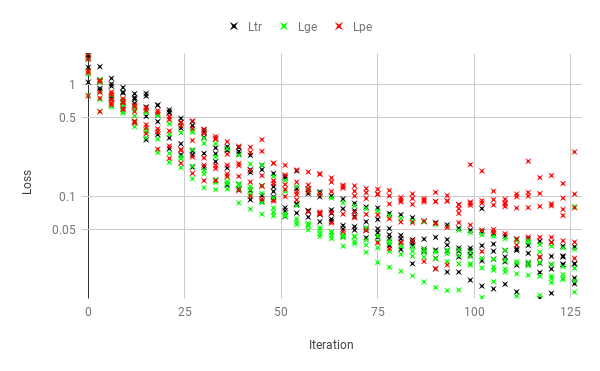
\includegraphics[width=.9\linewidth]{fig/content/results/shortest_path/epochs_base.png}
            \caption{Loss graphic with training set repeating on every 25 iterations, with permutations only of the testing set}
            \label{fig:shotest_paths_base_epochs_results}
        \end{figure}
        
        \begin{figure}[H]
            \centering
            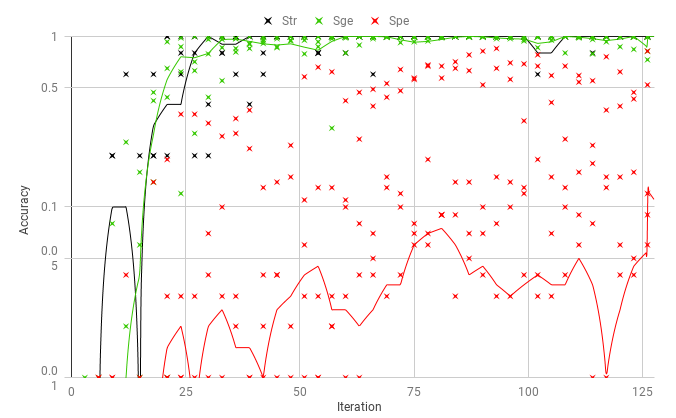
\includegraphics[width=.9\linewidth]{fig/content/results/shortest_path/epochs_base_ACC.png}
            \caption{Accuracy graphic with training set repeating on every 25 iterations, with permutations only of the testing set}
            \label{fig:shotest_paths_base_epochs_ACC_results}
        \end{figure}

    \end{enumerate}

\subsubsection {Permutation of the training and testing sets}

\begin{enumerate}[label=(\Alph*)]

        \item Infinite dataset
        
        The difference from the subsection 5.2.1 \ref{sec:infinite_test_only} is that now we permuted the training set as well.
        
        The loss of the permuted testing set in (Fig.\ref{fig:shotest_paths_train_perm_results}) is lower than in (Fig.\ref{fig:shotest_paths_base_results}). The permuted testing set's loss trend converges with the non-permuted testing set's loss trend.
        
        The Accuracy graphic (Fig.\ref{fig:shotest_paths_train_perm_ACC_results}) also shows an improvement in the networks' learning. We can see that now the network learns to identify the shortest path on the permuted testing set (the trend of the permuted testing set's accuracy reaches 1).
        
        \begin{figure}[H]
            \centering
            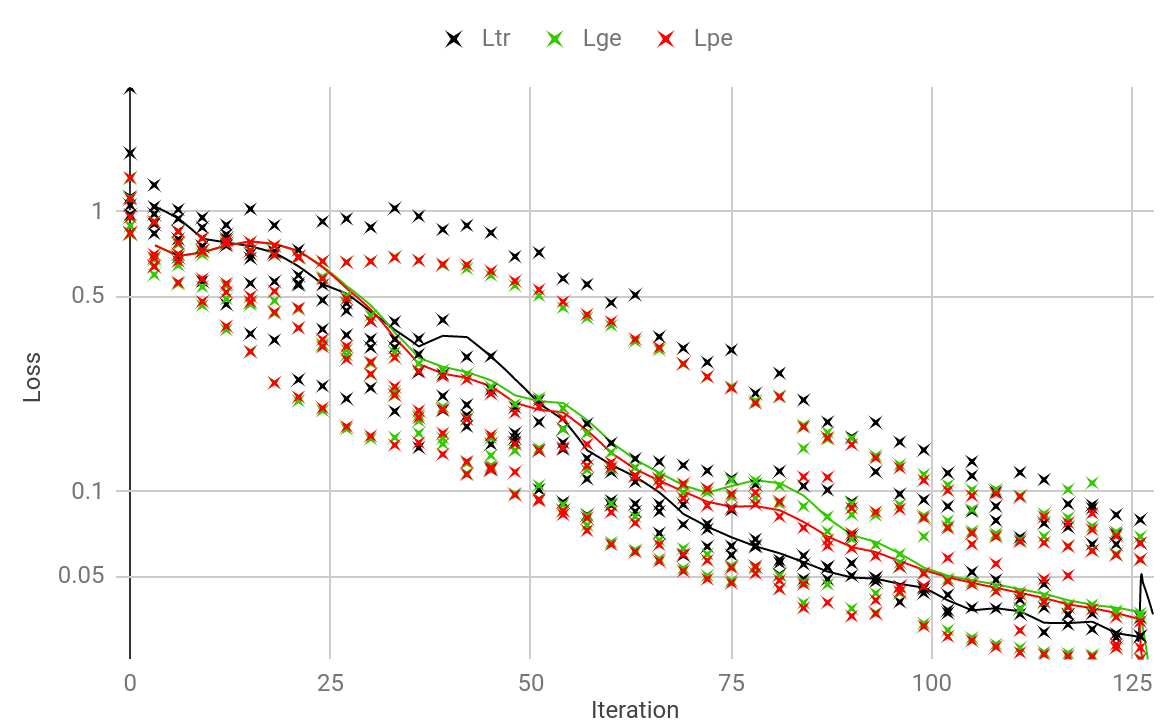
\includegraphics[width=.9\linewidth]{fig/content/results/shortest_path/training_perm.png}
            \caption{Loss graphic with infinite permuted training set}
            \label{fig:shotest_paths_train_perm_results}
        \end{figure}
        
        \begin{figure}[H]
            \centering
            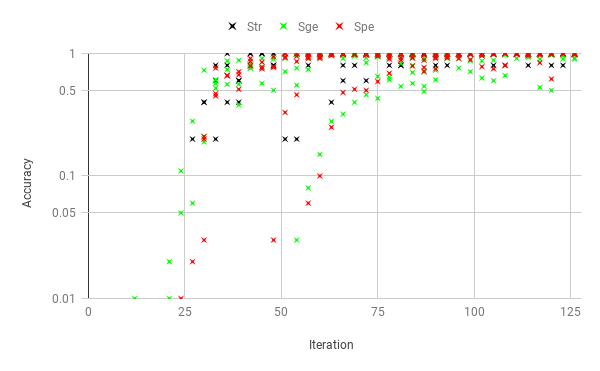
\includegraphics[width=.9\linewidth]{fig/content/results/shortest_path/training_perm_ACC.png}
            \caption{Accuracy graphic with infinite permuted training set}
            \label{fig:shotest_paths_train_perm_ACC_results}
        \end{figure}
        
        \item With epochs (every 25 iterations)
        
        The difference from the subsection 5.2.1 \ref{sec:epochs_test_only} is that now we permuted the training set as well.
        
        The Loss graphic (Fig.\ref{fig:shotest_paths_epochs_perm_results}) shows that the trend of the loss of the permuted testing set also converges with the trend of the loss of the non-permuted testing set, similar to (Fig. \ref{fig:shotest_paths_train_perm_results}).
        
        This similarity is also seen in the Accuracy graphic (Fig.\ref{fig:shotest_paths_epochs_perm_ACC_results}). The network learns to identify the shortest path on the permuted testing set (the trend of the permuted testing set's accuracy reaches 1).
        
        \begin{figure}[H]
            \centering
            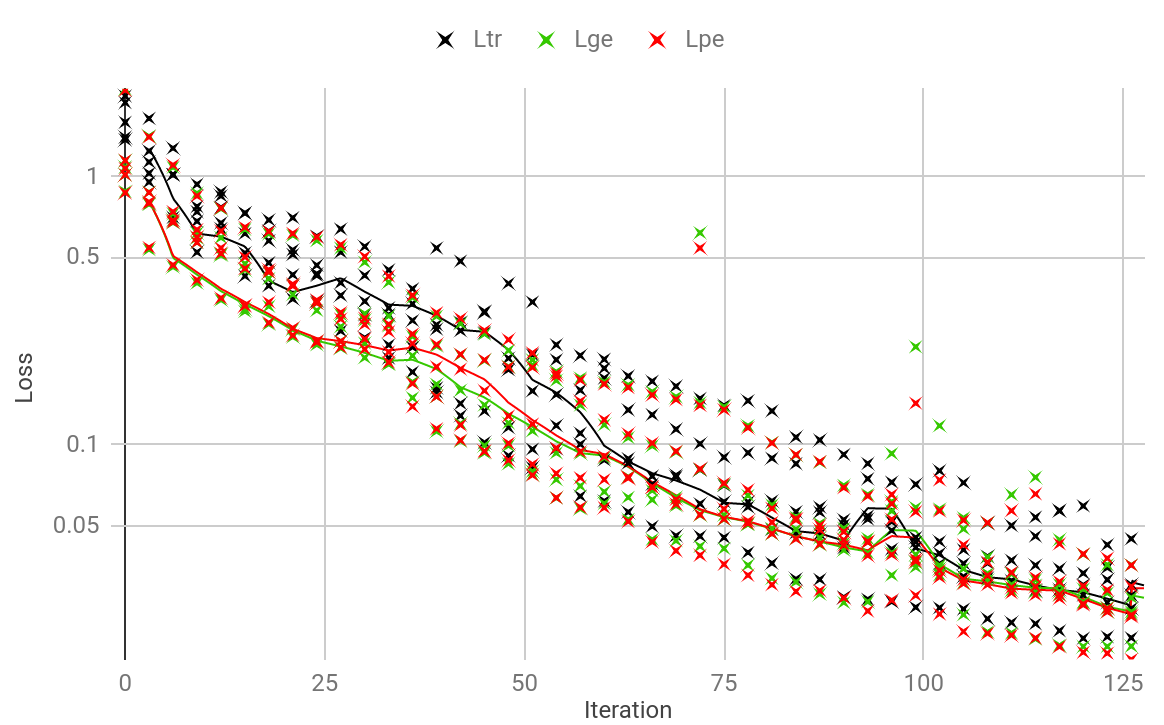
\includegraphics[width=.9\linewidth]{fig/content/results/shortest_path/epochs_perm.png}
            \caption{Loss graphic with permuted training set repeating on every 25 iterations}
            \label{fig:shotest_paths_epochs_perm_results}
        \end{figure}
        
        \begin{figure}[H]
            \centering
            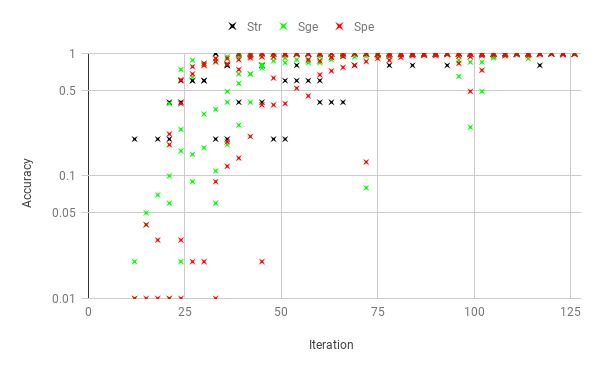
\includegraphics[width=.9\linewidth]{fig/content/results/shortest_path/epochs_perm_ACC.png}
            \caption{Accuracy graphic with permuted training set repeating on every 25 iterations}
            \label{fig:shotest_paths_epochs_perm_ACC_results}
        \end{figure}
        
        \item Various permutations of the same training set (per epoch)
        
        A limited dataset were used for the training set, the SEED were reset on every 25 iterations, generating epochs. But now, on every iteration we generate a different permutation of the same dataset and train the network with it.
        
        Since we are training with different permutations of the same dataset, we expected the network to learn how to deal with permutations faster, but it does not seem to be the case (as we can see in the Loss graphic from Fig.\ref{fig:shotest_paths_varios_perms_results}, which is very similar to the Loss graphic from Fig.\ref{fig:shotest_paths_epochs_perm_results}).
        
        However, in the Accuracy graphic (Fig.\ref{fig:shotest_paths_varios_perms_ACC_results}) the trends start to increase earlier compared to the Accuracy graphic from Fig.\ref{fig:shotest_paths_epochs_perm_ACC_results}. The network learns to identify the shortest path on the permuted testing set (the trend of the permuted testing set's accuracy reaches 1), as well.
        
        \begin{figure}[H]
            \centering
            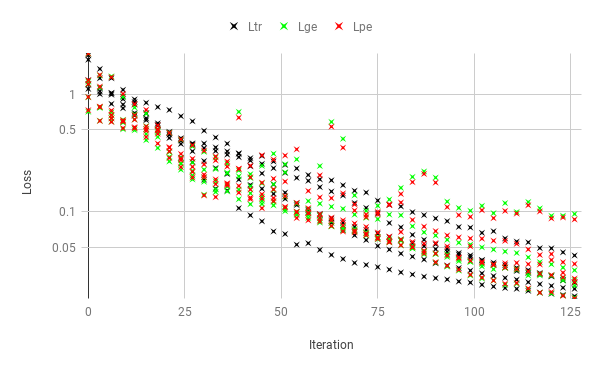
\includegraphics[width=.9\linewidth]{fig/content/results/shortest_path/various_perms_per_epoch.png}
            \caption{Loss graphic training with various permutations per epoch}
            \label{fig:shotest_paths_varios_perms_results}
        \end{figure}
        
        \begin{figure}[H]
            \centering
            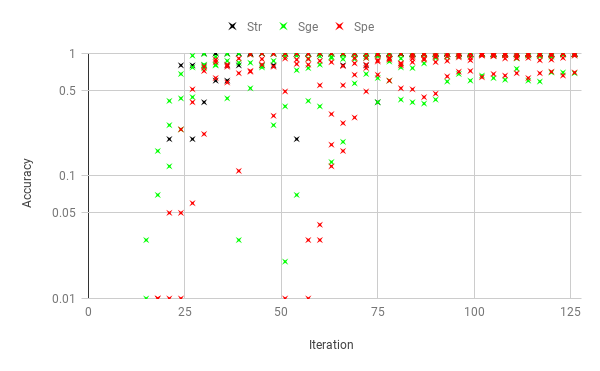
\includegraphics[width=.9\linewidth]{fig/content/results/shortest_path/various_perms_per_epoch_ACC.png}
            \caption{Accuracy graphic training with various permutations per epoch}
            \label{fig:shotest_paths_varios_perms_ACC_results}
        \end{figure}

    \end{enumerate}
    
\subsection{Experiments C - Regions Separation}
% \begin{figure}[H]
%     \centering
%     \subfigure[Testing in graphs with and without representational permutations]{
%         \includegraphics[width=.9\linewidth]{fig/content/results/shapes/base.png}
%     }
%     \subfigure[Same but permuting the training set as well]{
%         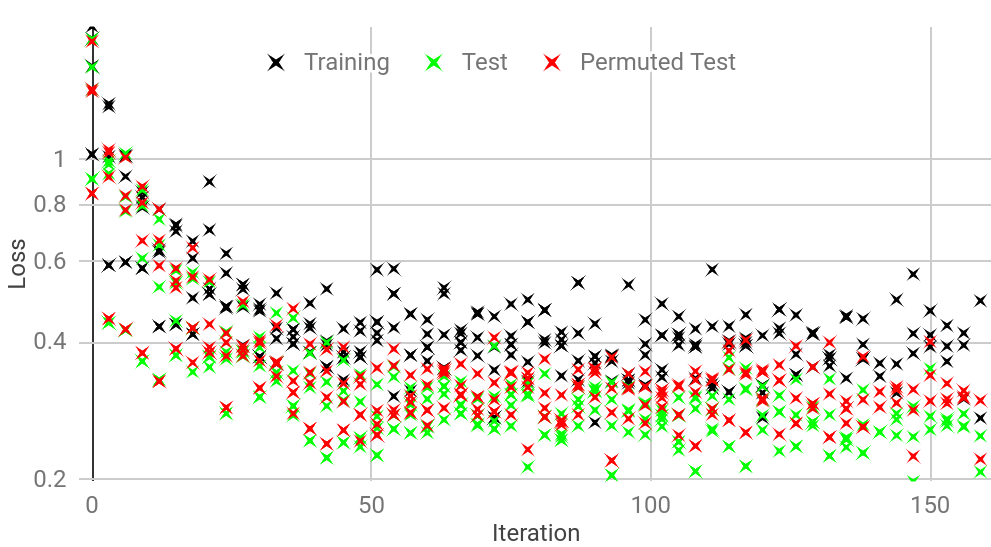
\includegraphics[width=.9\linewidth]{fig/content/results/shapes/ptr.png}
%     }
%     \caption{Influence of representational permutations in test and train sets}
%     \label{fig:regions_separation_results}
% \end{figure}

The results of the experiments described before were plotted separating the cases of permuted (Fig.\ref{fig:regions_separation_permuting_training_loss}) and non-permuted (Fig.\ref{fig:regions_separation_base_loss}) training and for each one, separating the loss of test/generalization with permutations in the test set (pe) and without them (ge).

\subsubsection {Permutation of the testing set}

\begin{figure}[H]
    \centering
    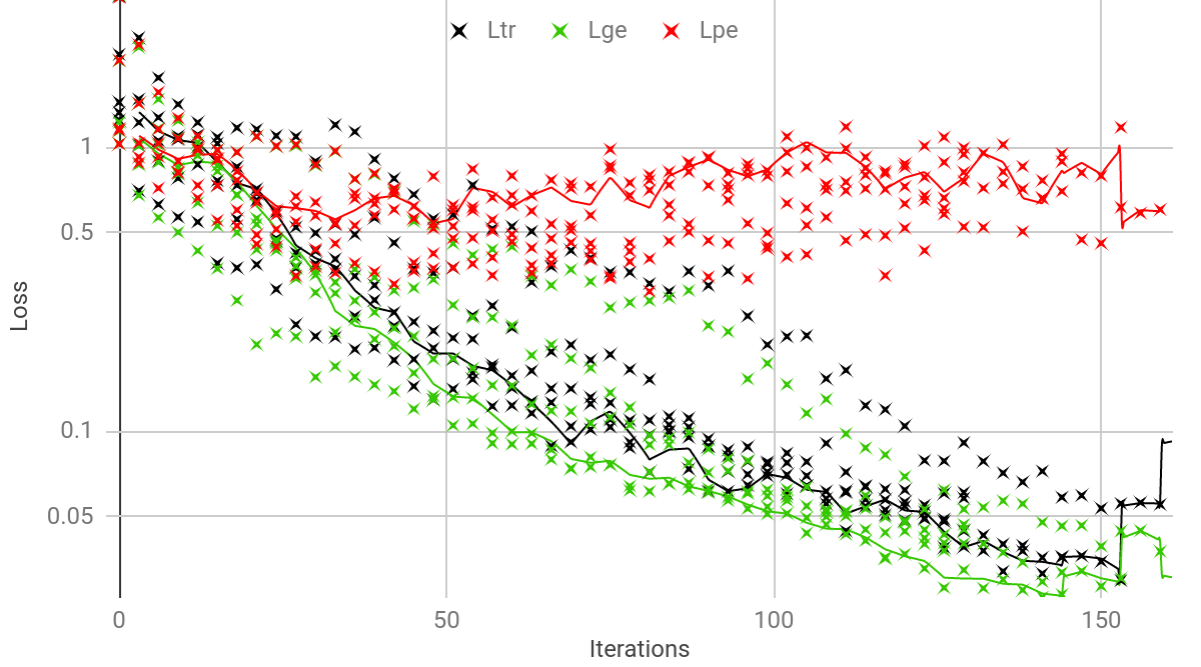
\includegraphics[width=.9\linewidth]
    {fig/content/results/shapes/base/loss.png}
    \caption{Loss plot of the experiments without permutations in the training set}
    \label{fig:regions_separation_base_loss}
\end{figure}

Without permutations in the data structure representation of the graphs in the training set, we can observe a clear separation between the loss of test with (Lpe) and without (Lge) permutations in the representation, which suggests, at least in this case, that in this framework, the algorithm is not invariant with respect to those permutations in the data structure representation of the graphs.

\begin{figure}[H]
    \centering
    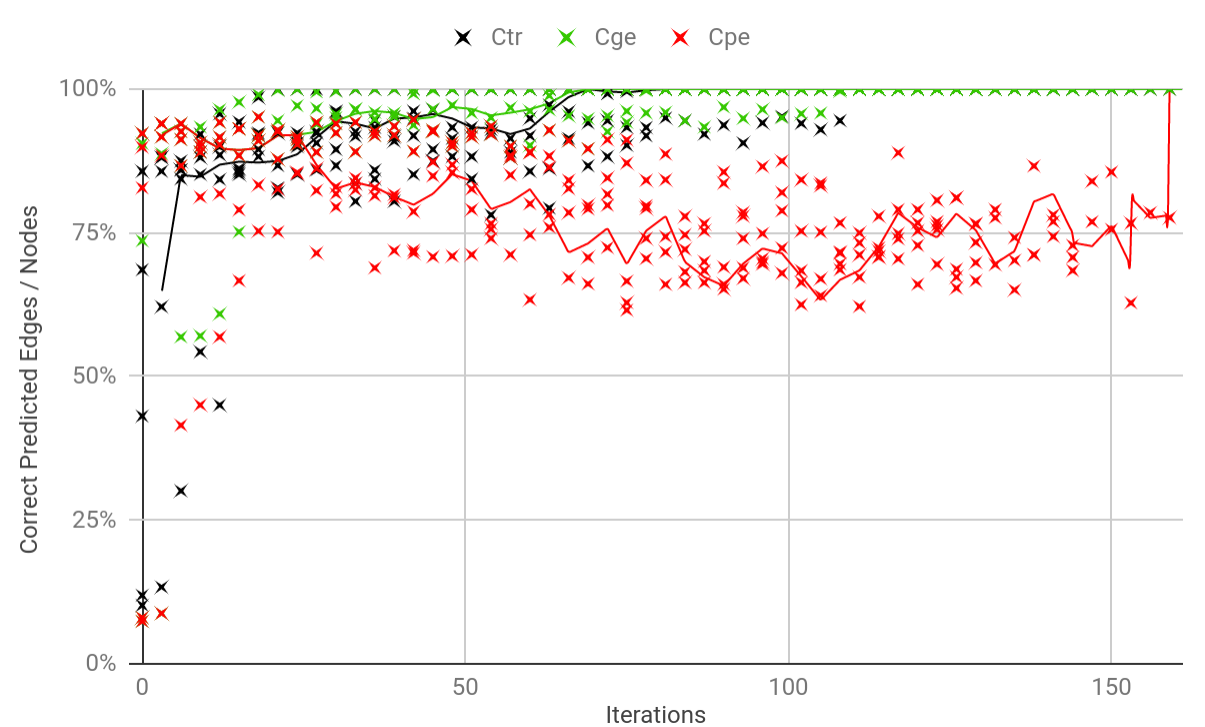
\includegraphics[width=.9\linewidth]
    {fig/content/results/shapes/base/correct.png}
    \caption{Accuracy plot of the experiments without permutations in the training set}
    \label{fig:regions_separation_base_accuracy}
\end{figure}

Analysing the accuracy plot considering the proportion of correct predicted nodes and edges (Fig.\ref{fig:regions_separation_base_accuracy}) in the case without permutations in the training set, we can see that Cge reached 100\% but Cpe didn't. In fact accuracy slightly decreases after the first peak.

\subsubsection {Permutation of the training and testing sets}

\begin{figure}[H]
    \centering
    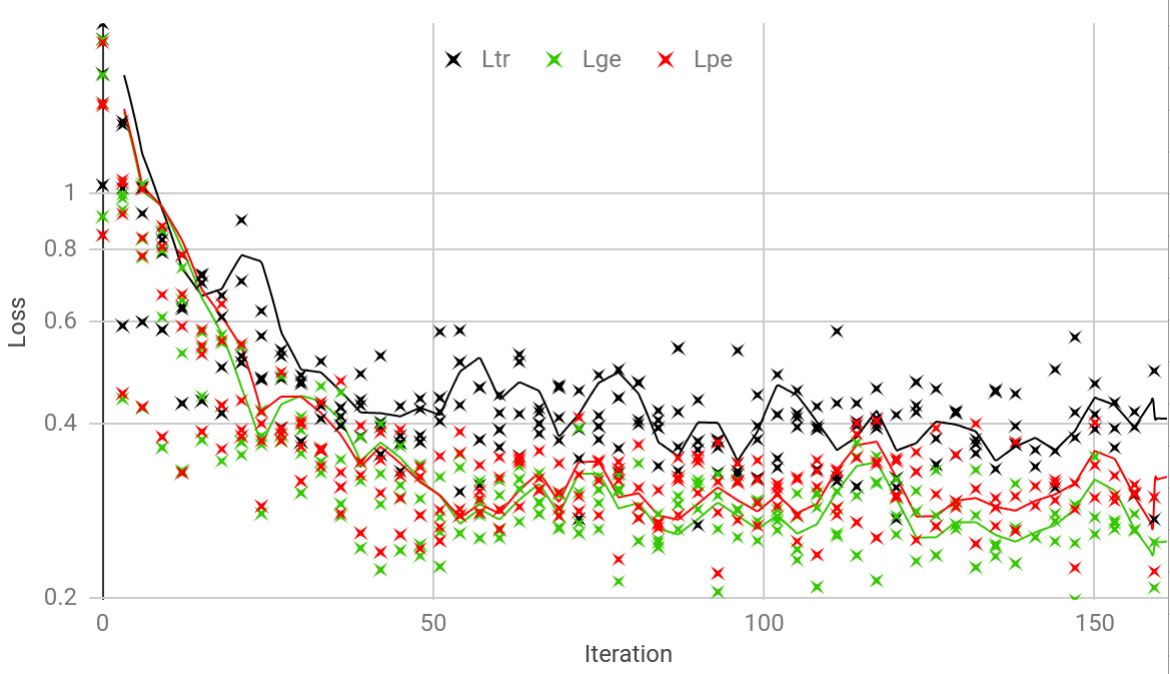
\includegraphics[width=.9\linewidth]
    {fig/content/results/shapes/permuted_training/loss.png}
    \caption{Loss graphic of the experiment with permutations in the training set}
    \label{fig:regions_separation_permuting_training_loss}
\end{figure}

Permuting the representations of the training set, even though the difference between Lge and Lpe is greatly reduced in comparison with the previous experiment (without permutations in training), we can see that no loss gets below 0.2 when in the previous one, they get below 0.05 which suggests a significant reduction in the performance of the network.

\begin{figure}[H]
    \centering
    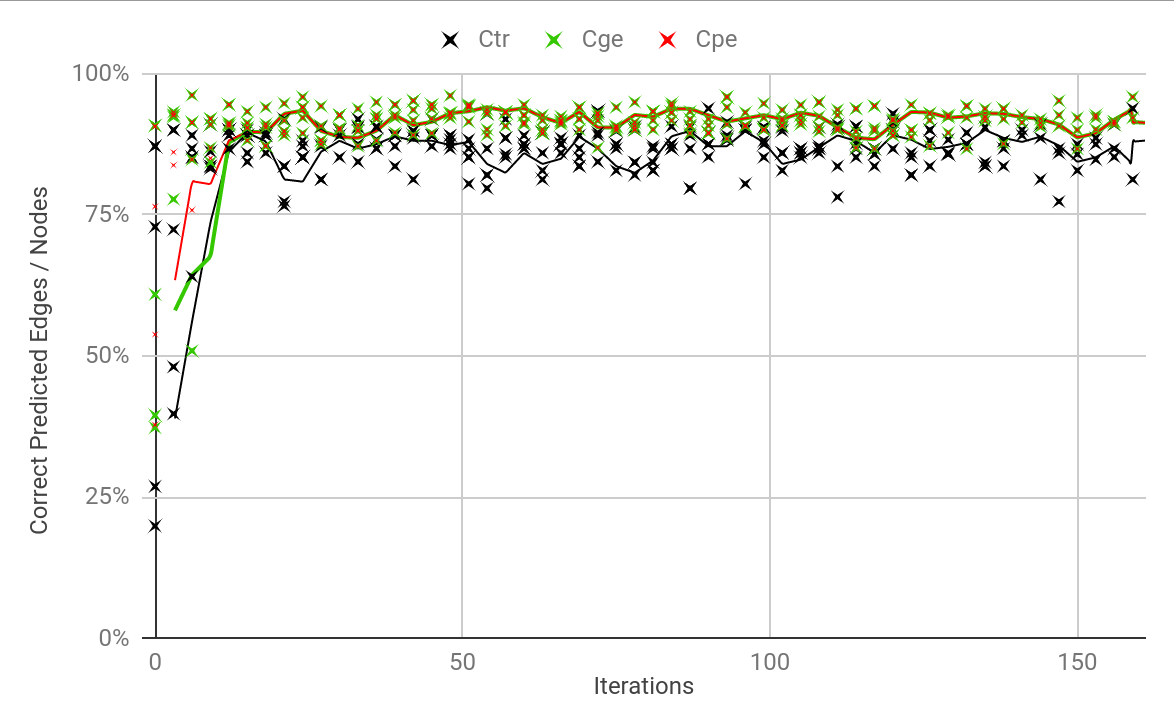
\includegraphics[width=.9\linewidth]
    {fig/content/results/shapes/permuted_training/correct.png}
    \caption{Accuracy graphic of the experiment with permutations in the training set}
    \label{fig:regions_separation_permuting_training_accuracy}
\end{figure}

Analysing the accuracy plot (Fig. \ref{fig:regions_separation_permuting_training_accuracy}) in the case with permutations in the training set, we can see that nor Cpe neither Cge reach 100\%, which means that none of them actually learned to solve the problem in the time box available. 



